% Graphics for slide 27, in the order the PDF draws them.
\begin{tikzpicture}[remember picture, overlay, x=1bp, y=-1bp,
  shift={(current page.north west)}]
\path[fill=cFFFFFF] (0,0) rectangle (960,540);
\node[anchor=north west, inner sep=0pt] at (56.69,477.21) {
\includegraphics[width=73.42bp, height=37.42bp]{figures/fundamentals-of-hpc/p03-1.png}};
\path[fill=cEE7628,even odd rule] (57.18,55.73) ..controls(57.96,55.73)and(58.6,56.37)..(58.6,57.15) --(58.6,85.5) ..controls(58.6,86.28)and(57.96,86.91)..(57.18,86.91) ..controls(56.4,86.91)and(55.76,86.28)..(55.76,85.5) --(55.76,57.15) ..controls(55.76,56.37)and(56.4,55.73)..(57.18,55.73);
\node[anchor=north west, inner sep=0pt] at (572.99,243.51) {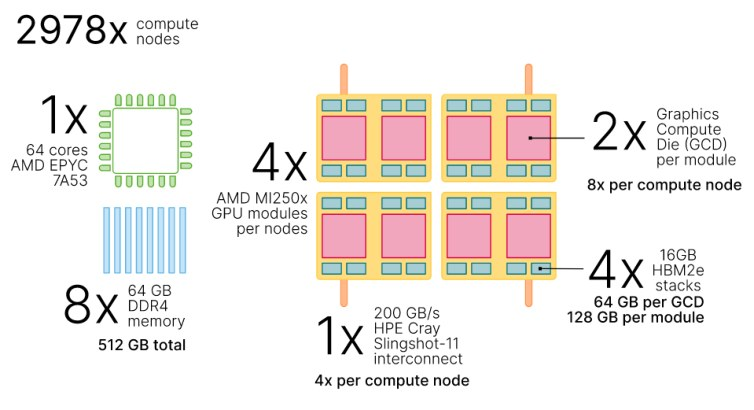
\includegraphics[width=251.01bp, height=136.37bp]{figures/fundamentals-of-hpc/p27-2.jpg}};
\node[anchor=north west, inner sep=0pt] at (567.39,43.48) {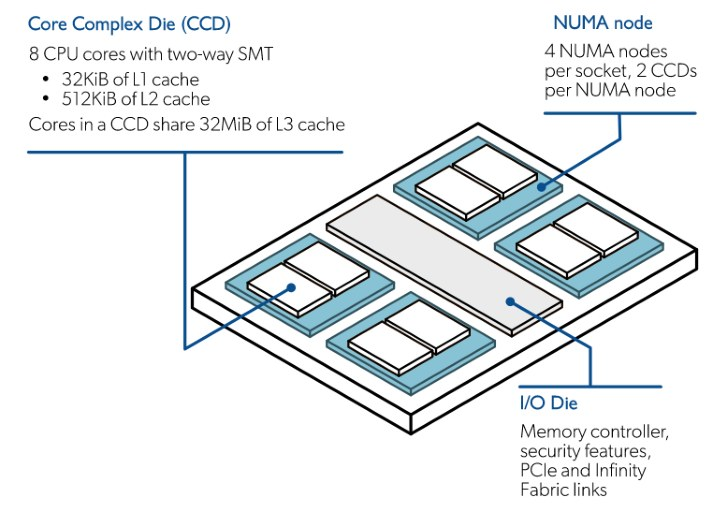
\includegraphics[width=237.55bp, height=175.51bp]{figures/fundamentals-of-hpc/p27-3.jpg}};
\node[anchor=north west, inner sep=0pt] at (587.49,402.79) {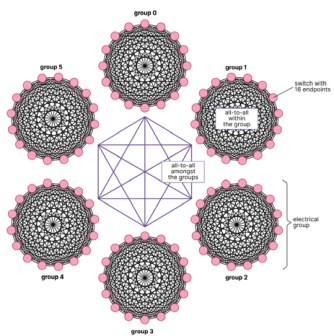
\includegraphics[width=111.1bp, height=111.84bp]{figures/fundamentals-of-hpc/p27-4.jpg}};
\end{tikzpicture}
